% Compile with XeLaTeX. Chinese version requires Noto Sans CJK SC.
\documentclass[tikz,border=4pt]{standalone}
\usepackage{fontspec,amsmath,amssymb}
\setmainfont{DejaVu Sans}
\usetikzlibrary{arrows.meta,calc}
\definecolor{paper}{HTML}{FCFBF8}
\definecolor{panel}{HTML}{F3F1EC}
\definecolor{ink}{HTML}{292A28}
\definecolor{muted}{HTML}{696B65}
\definecolor{pku}{HTML}{842C36}
\definecolor{sage}{HTML}{526B60}
\begin{document}
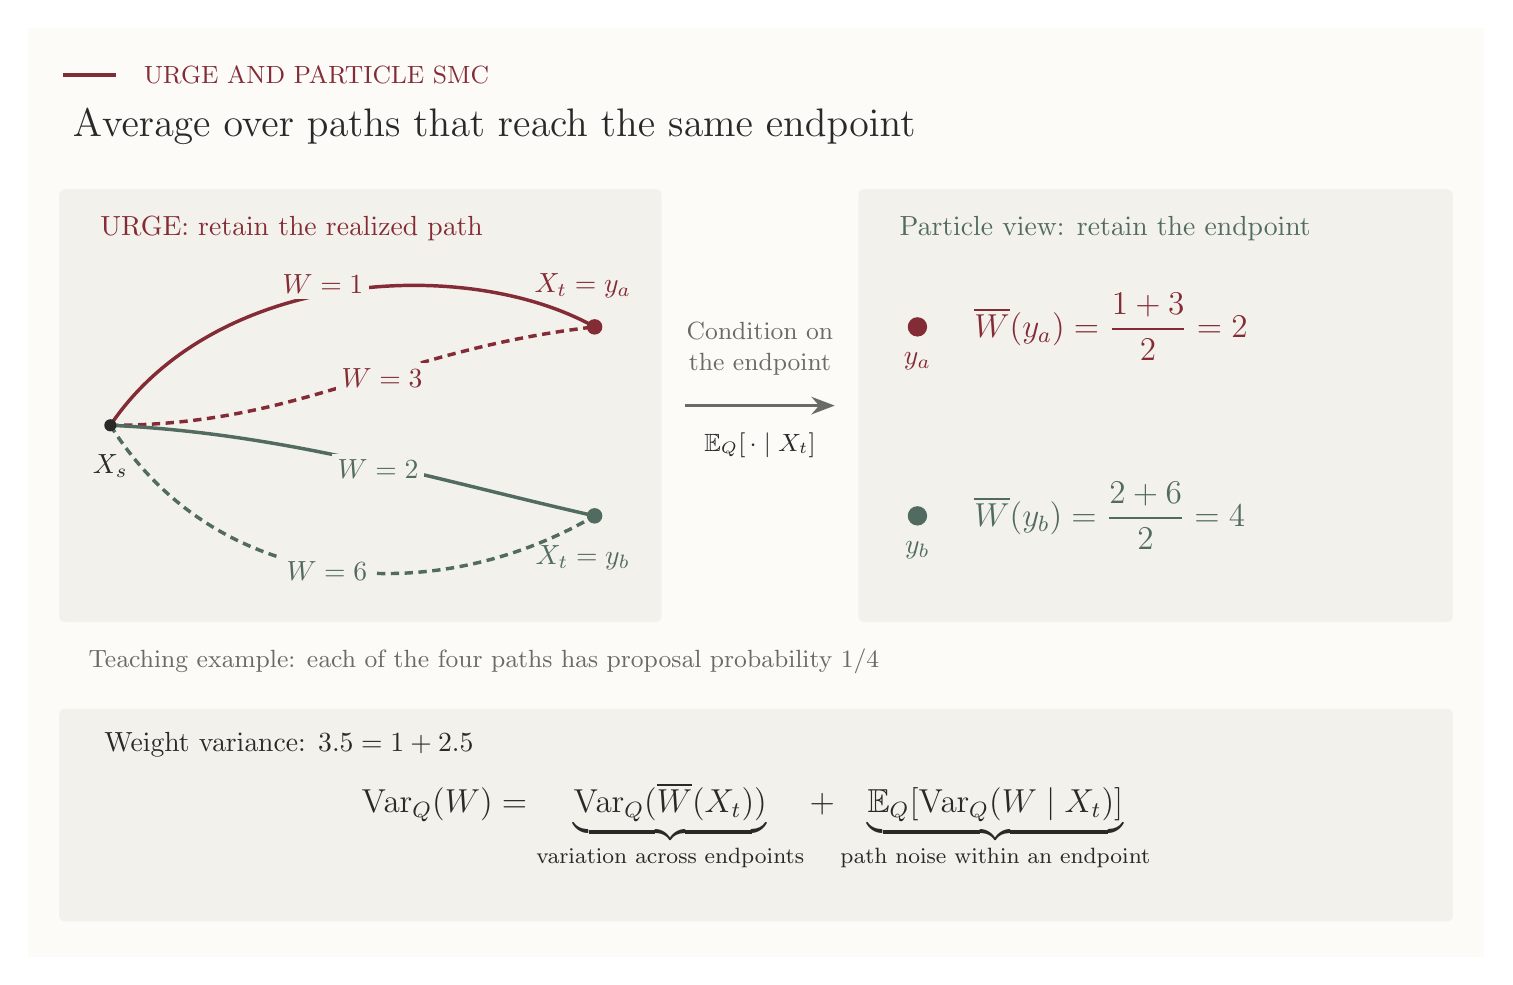
\begin{tikzpicture}[x=1cm,y=1cm,font=\small,text=ink,>=Stealth]
\fill[paper] (0,0) rectangle (18.5,11.8);
\draw[pku,line width=1.4pt] (.45,11.2)--(1.12,11.2);
\node[anchor=west,text=pku,font=\small] at (1.35,11.2) {URGE AND PARTICLE SMC};
\node[anchor=west,font=\Large] at (.45,10.55) {Average over paths that reach the same endpoint};
\fill[panel,rounded corners=2pt] (.4,4.25) rectangle (8.05,9.75);
\fill[panel,rounded corners=2pt] (10.55,4.25) rectangle (18.1,9.75);
\node[anchor=west,text=pku,font=\normalsize] at (.8,9.25) {URGE: retain the realized path};
\node[anchor=west,text=sage,font=\normalsize] at (10.95,9.25) {Particle view: retain the endpoint};
\coordinate (start) at (1.05,6.75);
\coordinate (a) at (7.2,8.0);
\coordinate (b) at (7.2,5.6);
\draw[pku,line width=1.25pt] (start) .. controls (2.4,8.75) and (5.6,8.9) .. (a);
\draw[pku,line width=1.25pt,densely dashed] (start) .. controls (3.5,6.75) and (4.6,7.7) .. (a);
\draw[sage,line width=1.25pt] (start) .. controls (3.3,6.65) and (5.2,6.05) .. (b);
\draw[sage,line width=1.25pt,densely dashed] (start) .. controls (2.4,4.6) and (5.15,4.4) .. (b);
\fill[ink] (start) circle (2.2pt);
\fill[pku] (a) circle (2.8pt);
\fill[sage] (b) circle (2.8pt);
\node[anchor=north,font=\normalsize] at (1.05,6.5) {$X_s$};
\node[anchor=south,text=pku,font=\normalsize] at (7.05,8.25) {$X_t=y_a$};
\node[anchor=north,text=sage,font=\normalsize] at (7.05,5.35) {$X_t=y_b$};
\node[text=pku,fill=panel,inner sep=2pt,font=\normalsize] at (3.75,8.55) {$W=1$};
\node[text=pku,fill=panel,inner sep=2pt,font=\normalsize] at (4.5,7.35) {$W=3$};
\node[text=sage,fill=panel,inner sep=2pt,font=\normalsize] at (4.45,6.2) {$W=2$};
\node[text=sage,fill=panel,inner sep=2pt,font=\normalsize] at (3.8,4.9) {$W=6$};
\draw[->,muted,line width=1.2pt] (8.35,7.0)--(10.25,7.0);
\node[align=center,text=muted,font=\small] at (9.3,7.72) {Condition on\\the endpoint};
\node[font=\small] at (9.3,6.5) {$\mathbb E_Q[\,\cdot\mid X_t]$};
\fill[pku] (11.3,8) circle (3.5pt);
\fill[sage] (11.3,5.6) circle (3.5pt);
\node[text=pku,anchor=north,font=\normalsize] at (11.3,7.8) {$y_a$};
\node[text=sage,anchor=north,font=\normalsize] at (11.3,5.4) {$y_b$};
\node[anchor=west,text=pku,font=\large] at (11.9,8.0) {$\overline W(y_a)=\dfrac{1+3}{2}=2$};
\node[anchor=west,text=sage,font=\large] at (11.9,5.6) {$\overline W(y_b)=\dfrac{2+6}{2}=4$};
\node[anchor=west,text=muted,font=\small] at (.65,3.75) {Teaching example: each of the four paths has proposal probability $1/4$};
\fill[panel,rounded corners=2pt] (.4,.45) rectangle (18.1,3.15);
\node[anchor=west,font=\normalsize] at (.85,2.7) {Weight variance: $3.5=1+2.5$};
\node[font=\large] at (9.25,1.65) {$\operatorname{Var}_Q(W)
=\underbrace{\operatorname{Var}_Q(\overline W(X_t))}_{\text{variation across endpoints}}
+\underbrace{\mathbb E_Q[\operatorname{Var}_Q(W\mid X_t)]}_{\text{path noise within an endpoint}}$};
\end{tikzpicture}
\end{document}
